\chapter{ANÁLISIS Y DISCUSIÓN DE RESULTADOS}
Como parte de la aplicación de la metodología CRISP-DM, explicada en el sexto subcapítulo del Capítulo III, se mencionaron las métricas usadas en la literatura. La más recurrente fue la exactitud. Dado que la librería Scikit-learn cuenta con un reporte de clasificación con esta métrica y otras 4 más como la precisión, sensibilidad, puntaje F1 y AUC, además que la distribución de proyectos por su estado de financiamiento es desbalanceada y se necesita más de un indicador para poder evaluar y comparar, se decidió usar estas 5 teniendo como referencias a los autores \citeauthor{pr_beckwith2016predcrowd} (quinto antecedente), \citeauthor{pr_yuan2016textanalytics}* (séptimo antecedente), \citeauthor{pr_kaur2017socmedcrowd} (noveno antecedente), \citeauthor{pr_cheng2019deeplearning} (decimocuarto antecedente), y \citeauthor{pr_chen2019keywords_crowdfunding}** (decimoquinto antecedente).

En el antecedente marcado en (*), los modelos no fueron evaluados por AUC; mientras que en (**), las métricas precisión y AUC no fueron tomadas en cuenta.

\section{Metainformación}
Luego de 19 épocas, con un promedio de 3 segundos de entrenamiento cada una, el modelo dejó de entrenar dado que durante 7 épocas no registró una reducción en el valor de la pérdida del subconjunto de validación, a pesar de que hace 3 épocas se redujo su tasa de aprendizaje.

Así, de acuerdo a la Figura \ref{5:fig1}, en la época 11 se registran los mejores valores de exactitud y pérdida para el subconjunto de validación, alcanzando 0.9523 y 0.1246 respectivamente.

\begin{figure}[!ht]
	\begin{center}
		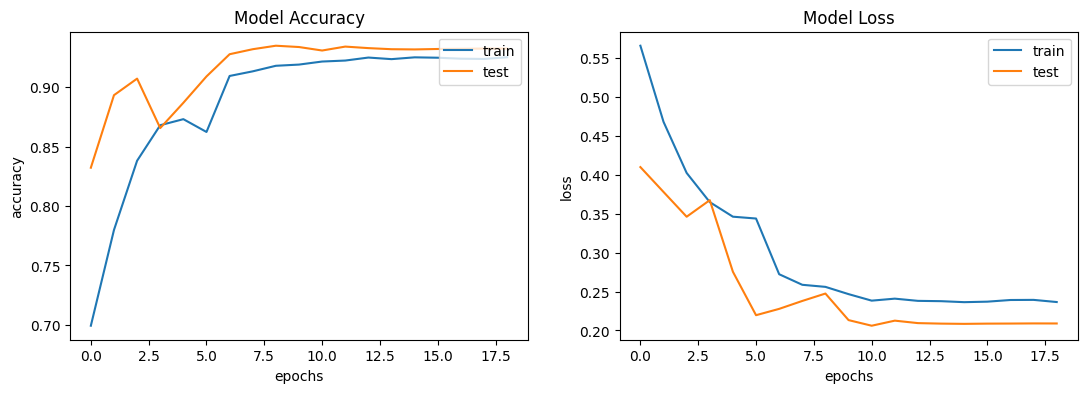
\includegraphics[width=1\textwidth]{5/figures/metadata_model_acc_loss.png}
		\caption[Exactitud y pérdida respectivamente de los subconjuntos de entrenamiento y validación para el modelo MLP de metadata con 100 épocas]{Exactitud y pérdida respectivamente de los subconjuntos de entrenamiento y validación para el modelo MLP de metadata con 100 épocas.\\
		Fuente: Elaboración propia.}
		\label{5:fig1}
	\end{center}
\end{figure}

La matriz de confusión resultante se representa en la Figura \ref{5:fig2}.

\begin{figure}[!ht]
	\begin{center}
		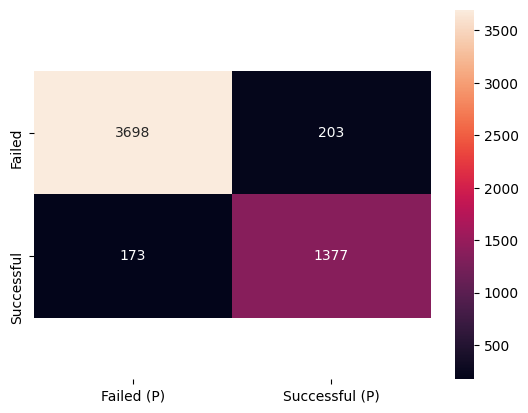
\includegraphics[width=0.60\textwidth]{5/figures/metadata_confusion_matrix.png}
		\caption[Matriz de confusión para el modelo de metadata]{Matriz de confusión para el modelo de metadata.\\
		Fuente: Elaboración propia.}
		\label{5:fig2}
	\end{center}
\end{figure}

De esta matriz, se derivan los resultados de la Tabla \ref{5:table1} y el AUC en la Figura \ref{5:fig3}.

\begin{table}[h!]
	\caption[Informe de clasificación para el modelo de metadata]{Informe de clasificación para el modelo de metadata.}
	\label{5:table1}
	\centering
	\small
	\begin{tabular}{ |m{4.5cm}|m{2.5cm}|m{2.5cm}|m{2.5cm}|m{2.5cm}|  }
		\hline
		%\rowcolor{bluejean}
		\Centering \textbf{Valor}& \Centering \textbf{Precisión}& \Centering \textbf{Sensibilidad}& \Centering \textbf{Puntaje F1}& \Centering \textbf{Muestras}\\
		\hline
		\textbf{Fracasado} & 0.96 & 0.95 & 0.95 & 3,901 \\
		\hline
		\textbf{Exitoso} & 0.87 & 0.89 & 0.88 & 1,550 \\
		\hline
		%\rowcolor{turq}
		\multicolumn{5}{c}{ } \\
		\hline
		\textbf{Exactitud} &  &	 & 0.93 & 5,451 \\
		\hline
		\textbf{Promedio macro} & 0.91 & 0.92 & 0.92 & 5,451 \\
		\hline
		\textbf{Promedio ponderado} & 0.93 & 0.93 & 0.93 & 5,451 \\
		\hline
	\end{tabular}
	\par	%%Salto de linea
	\bigskip
	\begin{flushleft}	%%Alinear a la izquierda sin justificar
		\small Fuente: Elaboración propia.
	\end{flushleft}
\end{table}

\begin{itemize}
	\item El ratio de exactitud se interpreta como: El 93\% de los proyectos de la muestra fueron predichos correctamente.
	\item El ratio de precisión para los positivos (\textit{Successful}) se interpreta como: El 87\% de los proyectos exitosos predichos de la muestra fueron clasificados correctamente. 
	\item El ratio de sensibilidad para los positivos (\textit{Successful}) se interpreta como: El 89\% de los proyectos exitosos reales de la muestra fueron clasificados correctamente.
	\item El ratio de Puntaje F1 para los positivos (\textit{Successful}) representa un balance entre las 2 métricas anteriores. En la tabla se observa que su valor es de 88\%, lo cual indica que en general, el modelo mantiene un alto rendimiento.
\end{itemize}

\begin{figure}[!ht]
	\begin{center}
		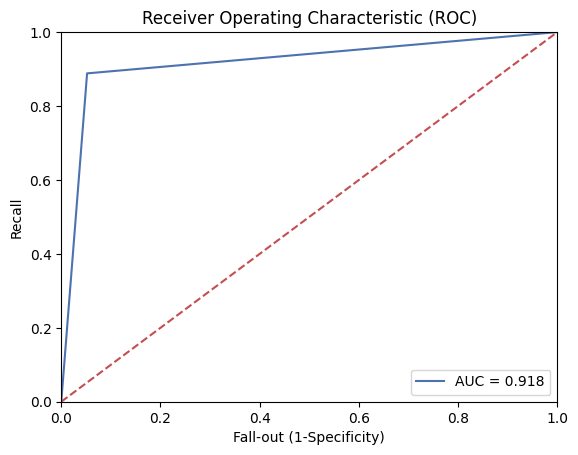
\includegraphics[width=0.55\textwidth]{5/figures/metadata_auc.png}
		\caption[Área bajo la curva ROC de modelo de metadata]{Área bajo la curva ROC de modelo de metadata.\\
		Fuente: Elaboración propia.}
		\label{5:fig3}
	\end{center}
\end{figure}

El área bajo la Curva ROC presenta un valor de aproximadamente 92\%, del cual se observa en el gráfico que su sensibilidad es muy alta y el ratio de Falsa Alarma o Falsos Positivos es casi nulo. Esto significa que el poder discriminante del modelo es excelente \parencite{bk_britos2006datamining}.

\section{Descripción}
Luego de 82 épocas, con un promedio de 106 segundos de entrenamiento cada una, el modelo dejó de entrenar dado que durante 10 épocas no registró una reducción en el valor de la pérdida del subconjunto de validación, a pesar de que hace 5 épocas se redujo su tasa de aprendizaje.

Así, de acuerdo a la Figura \ref{5:fig4}, en la época 72 se registran los mejores valores de exactitud y pérdida para el subconjunto de validación, alcanzando 0.7683 y 0.4901 respectivamente.

\begin{figure}[!ht]
	\begin{center}
		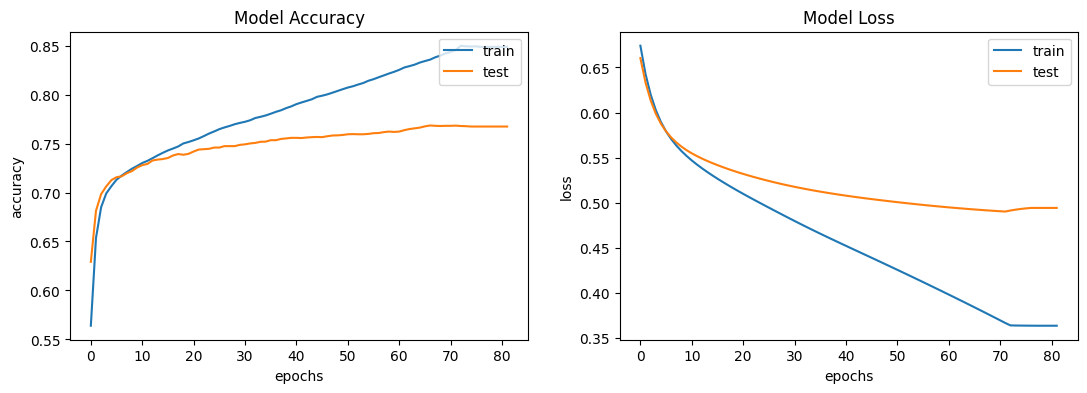
\includegraphics[width=1\textwidth]{5/figures/description_model_acc_loss.png}
		\caption[Exactitud y pérdida respectivamente de los subconjuntos de entrenamiento y validación para el modelo CNN de descripciones con 100 épocas]{Exactitud y pérdida respectivamente de los subconjuntos de entrenamiento y validación para el modelo CNN de descripciones con 100 épocas.\\
		Fuente: Elaboración propia.}
		\label{5:fig4}
	\end{center}
\end{figure}

La matriz de confusión resultante se representa en la Figura \ref{5:fig5}.

\begin{figure}[!ht]
	\begin{center}
		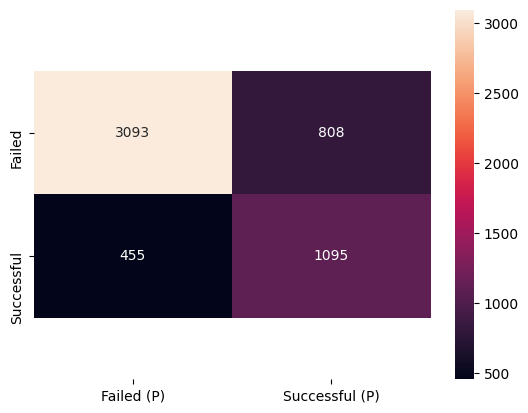
\includegraphics[width=0.60\textwidth]{5/figures/description_confusion_matrix.png}
		\caption[Matriz de confusión para el modelo de descripciones]{Matriz de confusión para el modelo de descripciones.\\
		Fuente: Elaboración propia.}
		\label{5:fig5}
	\end{center}
\end{figure}

De esta matriz, se derivan los resultados de la Tabla \ref{5:table2} y el AUC en la Figura \ref{5:fig6}.

\begin{table}[h!]
	\caption[Informe de clasificación para el modelo de descripciones]{Informe de clasificación para el modelo de descripciones.}
	\label{5:table2}
	\centering
	\small
	\begin{tabular}{ |m{4.5cm}|m{2.5cm}|m{2.5cm}|m{2.5cm}|m{2.5cm}|  }
		\hline
		%\rowcolor{bluejean}
		\Centering \textbf{Valor}& \Centering \textbf{Precisión}& \Centering \textbf{Sensibilidad}& \Centering \textbf{Puntaje F1}& \Centering \textbf{Muestras}\\
		\hline
		\textbf{Fracasado} & 0.87 & 0.79 & 0.83 & 3,901 \\
		\hline
		\textbf{Exitoso} & 0.58 & 0.71 & 0.63 & 1,550 \\
		\hline
		%\rowcolor{turq}
		\multicolumn{5}{c}{ } \\
		\hline
		\textbf{Exactitud} &  &	 & 0.77 & 5,451 \\
		\hline
		\textbf{Promedio macro} & 0.72 & 0.75 & 0.73 & 5,451 \\
		\hline
		\textbf{Promedio ponderado} & 0.79 & 0.77 & 0.77 & 5,451 \\
		\hline
	\end{tabular}
	\par	%%Salto de linea
	\bigskip
	\begin{flushleft}	%%Alinear a la izquierda sin justificar
		\small Fuente: Elaboración propia.
	\end{flushleft}
\end{table}

\begin{itemize}
	\item El ratio de exactitud se interpreta como: El 77\% de los proyectos de la muestra fueron predichos correctamente.
	\item El ratio de precisión para los positivos (\textit{Successful}) se interpreta como: El 58\% de los proyectos exitosos predichos de la muestra fueron clasificados correctamente. 
	\item El ratio de sensibilidad para los positivos (\textit{Successful}) se interpreta como: El 71\% de los proyectos exitosos reales de la muestra fueron clasificados correctamente.
	\item El ratio de Puntaje F1 para los positivos (\textit{Successful}) representa un balance entre las 2 métricas anteriores. En la tabla se observa que su valor es de 63\%, lo cual indica que en general, el modelo presenta un rendimiento regular.
\end{itemize}

\begin{figure}[!ht]
	\begin{center}
		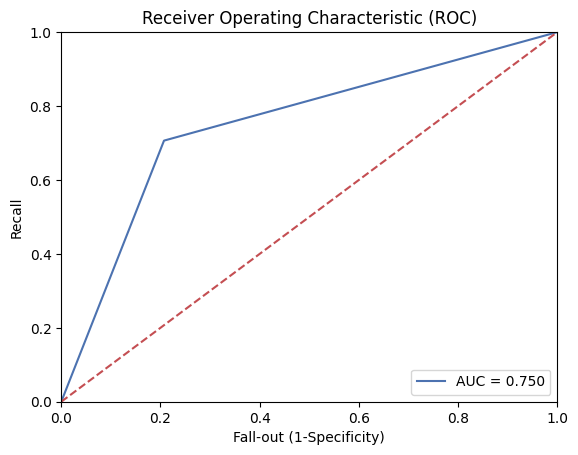
\includegraphics[width=0.55\textwidth]{5/figures/description_auc.png}
		\caption[Área bajo la curva ROC de modelo de descripciones]{Área bajo la curva ROC de modelo de descripciones.\\
		Fuente: Elaboración propia.}
		\label{5:fig6}
	\end{center}
\end{figure}

El área bajo la Curva ROC presenta un valor de aproximadamente 75\%, del cual se observa en el gráfico que su sensibilidad es medianamente alta y el ratio de Falsa Alarma es medianamente baja. Esto significa que el poder discriminante del modelo es aceptable \parencite{bk_britos2006datamining}.

\section{Comentarios}
Luego de 43 épocas, con 77 segundos en promedio de entrenamiento cada una, el modelo dejó de entrenar dado que durante 10 épocas no registró una reducción en el valor de la pérdida del subconjunto de validación, por más que 1 época antes se había reducido su tasa de aprendizaje.

Así, de acuerdo a la Figura \ref{5:fig7}, en la época 33 se registran los mejores valores de exactitud y pérdida para el subconjunto de validación, alcanzando 0.8510 y 0.4472 respectivamente.

\begin{figure}[!ht]
	\begin{center}
		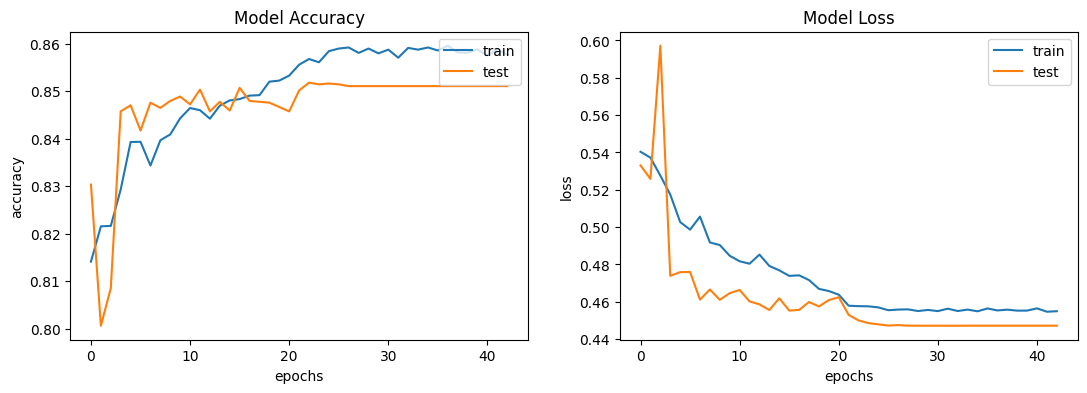
\includegraphics[width=1\textwidth]{5/figures/comments_model_acc_loss.png}
		\caption[Exactitud y pérdida respectivamente de los subconjuntos de entrenamiento y validación para el modelo RNN de comentarios con 50 épocas]{Exactitud y pérdida respectivamente de los subconjuntos de entrenamiento y validación para el modelo RNN de comentarios con 50 épocas.\\
		Fuente: Elaboración propia.}
		\label{5:fig7}
	\end{center}
\end{figure}

La matriz de confusión resultante se representa en la Figura \ref{5:fig8}.
\begin{figure}[!ht]
	\begin{center}
		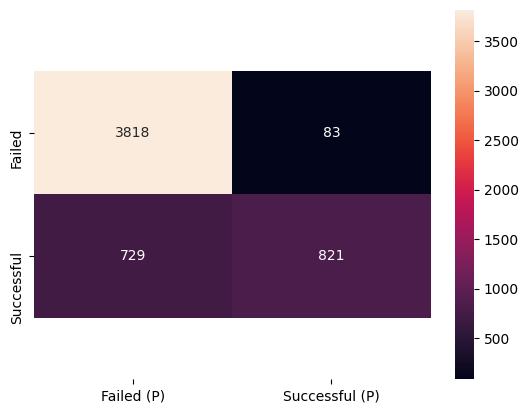
\includegraphics[width=0.60\textwidth]{5/figures/comments_confusion_matrix.png}
		\caption[Matriz de confusión para el modelo de comentarios]{Matriz de confusión para el modelo de comentarios.\\
		Fuente: Elaboración propia.}
		\label{5:fig8}
	\end{center}
\end{figure}

De esta matriz, se derivan los resultados de la Tabla \ref{5:table3} y el AUC en la Figura \ref{5:fig9}.

\begin{table}[h!]
	\caption[Informe de clasificación para el modelo de comentarios]{Informe de clasificación para el modelo de comentarios.}
	\label{5:table3}
	\centering
	\small
	\begin{tabular}{ |m{4.5cm}|m{2.5cm}|m{2.5cm}|m{2.5cm}|m{2.5cm}|  }
		\hline
		%\rowcolor{bluejean}
		\Centering \textbf{Valor}& \Centering \textbf{Precisión}& \Centering \textbf{Sensibilidad}& \Centering \textbf{Puntaje F1}& \Centering \textbf{Muestras}\\
		\hline
		\textbf{Fracasado} & 0.84 & 0.98 & 0.90 & 3,901 \\
		\hline
		\textbf{Exitoso} & 0.91 & 0.53 & 0.67 & 1,550 \\
		\hline
		%\rowcolor{turq}
		\multicolumn{5}{c}{ } \\
		\hline
		\textbf{Exactitud} &  &	 & 0.85 & 5,451 \\
		\hline
		\textbf{Promedio macro} & 0.87 & 0.75 & 0.79 & 5,451 \\
		\hline
		\textbf{Promedio ponderado} & 0.86 & 0.85 & 0.84 & 5,451 \\
		\hline
	\end{tabular}
	\par	%%Salto de linea
	\bigskip
	\begin{flushleft}	%%Alinear a la izquierda sin justificar
		\small Fuente: Elaboración propia.
	\end{flushleft}
\end{table}

\begin{itemize}
	\item El ratio de exactitud se interpreta como: El 85\% de los proyectos de la muestra fueron predichos correctamente.
	\item El ratio de precisión para los positivos (\textit{Successful}) se interpreta como: El 91\% de los proyectos exitosos predichos de la muestra fueron clasificados correctamente. 
	\item El ratio de sensibilidad para los positivos (\textit{Successful}) se interpreta como: El 53\% de los proyectos exitosos reales de la muestra fueron clasificados correctamente.
	\item El ratio de Puntaje F1 para los positivos (\textit{Successful}) representa un balance entre las 2 métricas anteriores. En la tabla se observa que su valor es de 67\%, lo cual indica que en general, el modelo presenta un rendimiento regular.
\end{itemize}

\begin{figure}[!ht]
	\begin{center}
		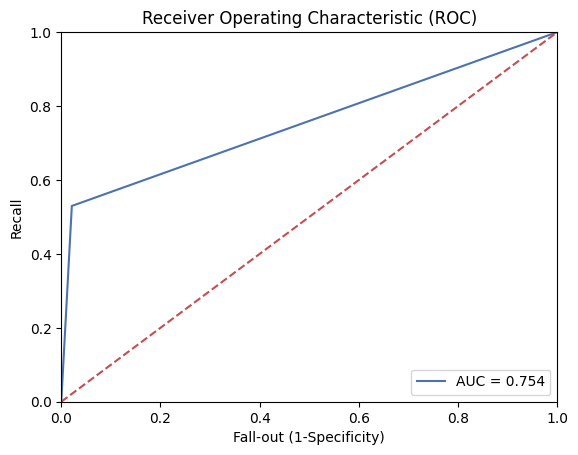
\includegraphics[width=0.55\textwidth]{5/figures/comments_auc.png}
		\caption[Área bajo la curva de modelo de comentarios]{Área bajo la curva de modelo de comentarios.\\
		Fuente: Elaboración propia.}
		\label{5:fig9}
	\end{center}
\end{figure}

El área bajo la Curva ROC presenta un valor de aproximadamente 75\%, del cual se observa en el gráfico que su sensibilidad es baja pero su ratio de Falsa Alarma es casi nulo. Esto significa que el poder discriminante del modelo es aceptable \parencite{bk_britos2006datamining}.

\section{Modelo apilado}
Luego de 13 épocas, con 152 segundos de entrenamientos cada una, el modelo dejó de entrenar dado que durante 10 épocas no registró una reducción en el valor de la pérdida del subconjunto de validación, a pesar de que hace 2 épocas se redujo su tasa de aprendizaje.

Así, de acuerdo a la Figura \ref{5:fig10}, en la época 3 se registran los mejores valores de exactitud y pérdida para el subconjunto de validación, alcanzando 0.9336 y 0.1810 respectivamente.

\begin{figure}[!ht]
	\begin{center}
		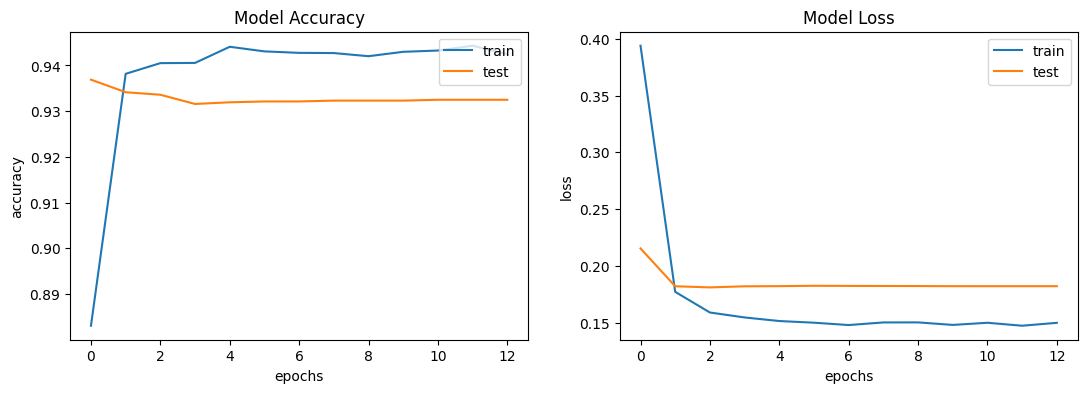
\includegraphics[width=1\textwidth]{5/figures/stacked_model_acc_loss.png}
		\caption[Exactitud y pérdida respectivamente de los subconjuntos de entrenamiento y validación para el modelo apilado con 200 épocas]{Exactitud y pérdida respectivamente de los subconjuntos de entrenamiento y validación para el modelo apilado con 200 épocas.\\
		Fuente: Elaboración propia.}
		\label{5:fig10}
	\end{center}
\end{figure}

La matriz de confusión resultante se representa en la Figura \ref{5:fig11}.
\begin{figure}[!ht]
	\begin{center}
		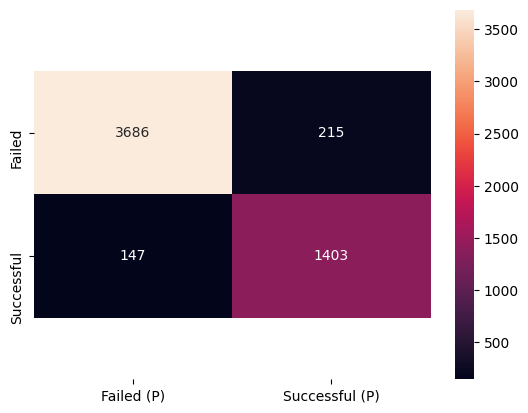
\includegraphics[width=0.55\textwidth]{5/figures/stacked_confusion_matrix.png}
		\caption[Matriz de confusión para el modelo apilado]{Matriz de confusión para el modelo apilado.\\
		Fuente: Elaboración propia.}
		\label{5:fig11}
	\end{center}
\end{figure}

De esta matriz, se derivan los resultados de la Tabla \ref{5:table4} y el AUC en la Figura \ref{5:fig12}.

\begin{table}[h!]
	\caption[Informe de clasificación para el modelo apilado]{Informe de clasificación para el modelo apilado.}
	\label{5:table4}
	\centering
	\small
	\begin{tabular}{ |m{4.5cm}|m{2.5cm}|m{2.5cm}|m{2.5cm}|m{2.5cm}|  }
		\hline
		%\rowcolor{bluejean}
		\Centering \textbf{Valor}& \Centering \textbf{Precisión}& \Centering \textbf{Sensibilidad}& \Centering \textbf{Puntaje F1}& \Centering \textbf{Muestras}\\
		\hline
		\textbf{Fracasado} & 0.96 & 0.94 & 0.95 & 3,901 \\
		\hline
		\textbf{Exitoso} & 0.87 & 0.91 & 0.89 & 1,550 \\
		\hline
		%\rowcolor{turq}
		\multicolumn{5}{c}{ } \\
		\hline
		\textbf{Exactitud} &  &	 & 0.93 & 5,451 \\
		\hline
		\textbf{Promedio macro} & 0.91 & 0.93 & 0.92 & 5,451 \\
		\hline
		\textbf{Promedio ponderado} & 0.93 & 0.93 & 0.93 & 5,451 \\
		\hline
	\end{tabular}
	\par	%%Salto de linea
	\bigskip
	\begin{flushleft}	%%Alinear a la izquierda sin justificar
		\small Fuente: Elaboración propia.
	\end{flushleft}
\end{table}

\begin{itemize}
	\item El ratio de exactitud se interpreta como: El 93\% de los proyectos de la muestra fueron predichos correctamente.
	\item El ratio de precisión para los positivos (\textit{Successful}) se interpreta como: El 87\% de los proyectos exitosos predichos de la muestra fueron clasificados correctamente. 
	\item El ratio de sensibilidad para los positivos (\textit{Successful}) se interpreta como: El 91\% de los proyectos exitosos reales de la muestra fueron clasificados correctamente.
	\item El ratio de Puntaje F1 para los positivos (\textit{Successful}) representa un balance entre las 2 métricas anteriores. En la tabla se observa que su valor es de 89\%, lo cual indica que en general, el modelo presenta un rendimiento regular.
\end{itemize}

\begin{figure}[!ht]
	\begin{center}
		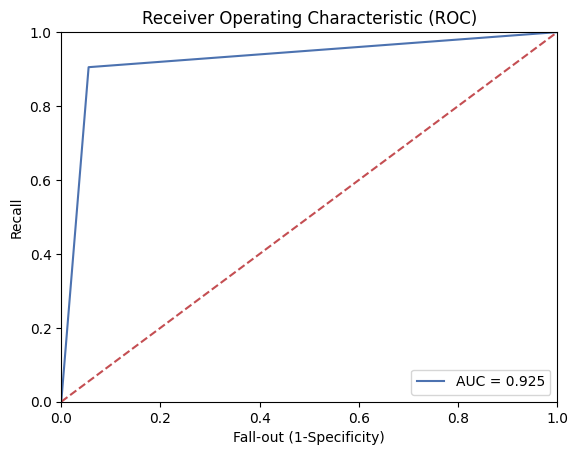
\includegraphics[width=0.50\textwidth]{5/figures/stacked_auc.png}
		\caption[Área bajo la curva de modelo apilado]{Área bajo la curva de modelo apilado.\\
		Fuente: Elaboración propia.}
		\label{5:fig12}
	\end{center}
\end{figure}

El área bajo la Curva ROC presenta un valor aproximado de 93\%, del cual se observa en el gráfico que su sensibilidad es muy alta y su ratio de Falsa Alarma es casi nulo. Esto significa que el poder discriminante del modelo es excepcionalmente bueno \parencite{bk_britos2006datamining}.

\section{Comparación de resultados}
Considerando los modelos independientes para cada modalidad, así como un trabajo previo del autor de la presente investigación cuyo trabajo sirvió de base \parencite{pr_puente2019kickstarter_prediction}, se armó el cuadro comparativo de la Tabla \ref{5:table5}.

\begin{table}[h!]
	\caption[Comparación de resultados de modelos propuestos con antecedentes]{Comparación de resultados de modelos propuestos con antecedentes.}
	\label{5:table5}
	\centering
	\small
	\begin{tabular}{|l|c|c|c|c|c|}
		\hline
		\multicolumn{1}{|c|}{\textbf{Modelos}} & {\textbf{Exactitud}} & {\textbf{Precisión}} & {\textbf{Sensibilidad}} & {\textbf{Puntaje F1}} & {\textbf{AUC}} \\ \hline
		Tesis de pregrado - Metainformación                                                            & 0.89                                                              & 0.86                                                              & 0.72                                                                 & 0.75                                                               & 0.84                                                        \\ \hline
		Tesis de pregrado - Descripción                                                         & 0.75                                                              & 0.59                                                              & 0.53                                                                 & 0.35                                                               & 0.68                                                        \\ \hline
		Propuesta - Metainformación                                                                  & 0.93                                                              & 0.91                                                              & 0.92                                                                 & 0.92                                                               & 0.92                                                        \\ \hline
		Propuesta - Descripción                                                               & 0.77                                                              & 0.72                                                              & 0.75                                                                 & 0.73                                                               & 0.75                                                        \\ \hline
		Propuesta - Comentarios                                                               & 0.85                                                              & 0.87                                                              & 0.75                                                                 & 0.79                                                               & 0.75                                                        \\ \hline
		\textbf{Propuesta - The Hydra}                                                        & \textbf{0.93}                                                     & \textbf{0.91}                                                     & \textbf{0.93}                                                        & \textbf{0.92}                                                      & \textbf{0.93}                                               \\ \hline
	\end{tabular}
	\par	%%Salto de linea
	\bigskip
	\begin{flushleft}	%%Alinear a la izquierda sin justificar
		\small Fuente: Elaboración propia.
	\end{flushleft}
\end{table}

Los modelos citados de la Tesis de pregrado para Metainformación y Descripción utilizaron una Máquina de Vectores de Soporte (SVM) y una SVM entrenada con el algoritmo TF-IDF, respectivamente.

Para comparar ambas investigaciones, se usaron las mismas bases de datos para las 2 modalidades, con proyectos tecnológicos de Kickstarter finalizados entre 2009 y 2019, así como también las mismas métricas para evaluar cada modelo. El tiempo de entrenamiento en el antecedente mencionado fue mayor (aproximadamente 16 segundos para la metainformación y 4 horas para la descripción), en contraste con los elaborados en este trabajo (aproximadamente 38 segundos para la metainformación y 2 horas y media para la descripción).

Como se observa en la Tabla \ref{5:table5}, a nivel general, la performance de The Hydra fue mejor tanto contra los modelos individuales de cada modalidad (superando en más de 0.03 y más de 0.05 al modelo de comentarios y descripción respectivamente en las 5 métricas, y en 0.01 al de metainformación en AUC) como contra los modelos referenciados en los antecedentes (más de 0.05 en todas las métricas para el modelo de metainformación y más de 0.18 en todas las métricas para el modelo de descripción). El concepto (con otros modelos y variantes en el desarrollo) utilizado en la Tesis de pregrado se basó en el trabajo de los autores \cite{pr_cheng2019deeplearning}, el cual utilizó un marco de trabajo de Aprendizaje Profundo Multimodal (\textit{Multimodal Deep Learning} en inglés), donde se combinan las características de metainformación, descripción e imagen principal del proyecto en la capa totalmente conectada. Sin embargo, en dicha ocasión no se alcanzó lograr los objetivos dado que el modelo de contenido visual presentó problemas para clasificar adecuadamente un proyecto según su estado. Esto se dio en parte a la variedad de imágenes dentro de la misma categoría Tecnología, que contiene asimismo 16 subcategorías, lo cual dificultó en su momento a la red a encontrar patrones a partir de su características. Se decidió, entonces, cambiar el criterio de reemplazar el contenido visual por otra modalidad respaldada por varios antecedentes (enunciados en la descripción del prototipo de investigación del Capítulo III) y que no fue tomada en cuenta en su momento, los comentarios realizados durante la campaña por los patrocinadores del proyecto.

\clearpage

\section{Demostración del modelo final}
Para culminar con la investigación, se diseñó un sistema piloto que logra predecir el estado de financiamiento de un determinado proyecto siguiendo el flujo de la Figura \ref{5:fig13}.

\begin{figure}[h]
	\begin{center}
		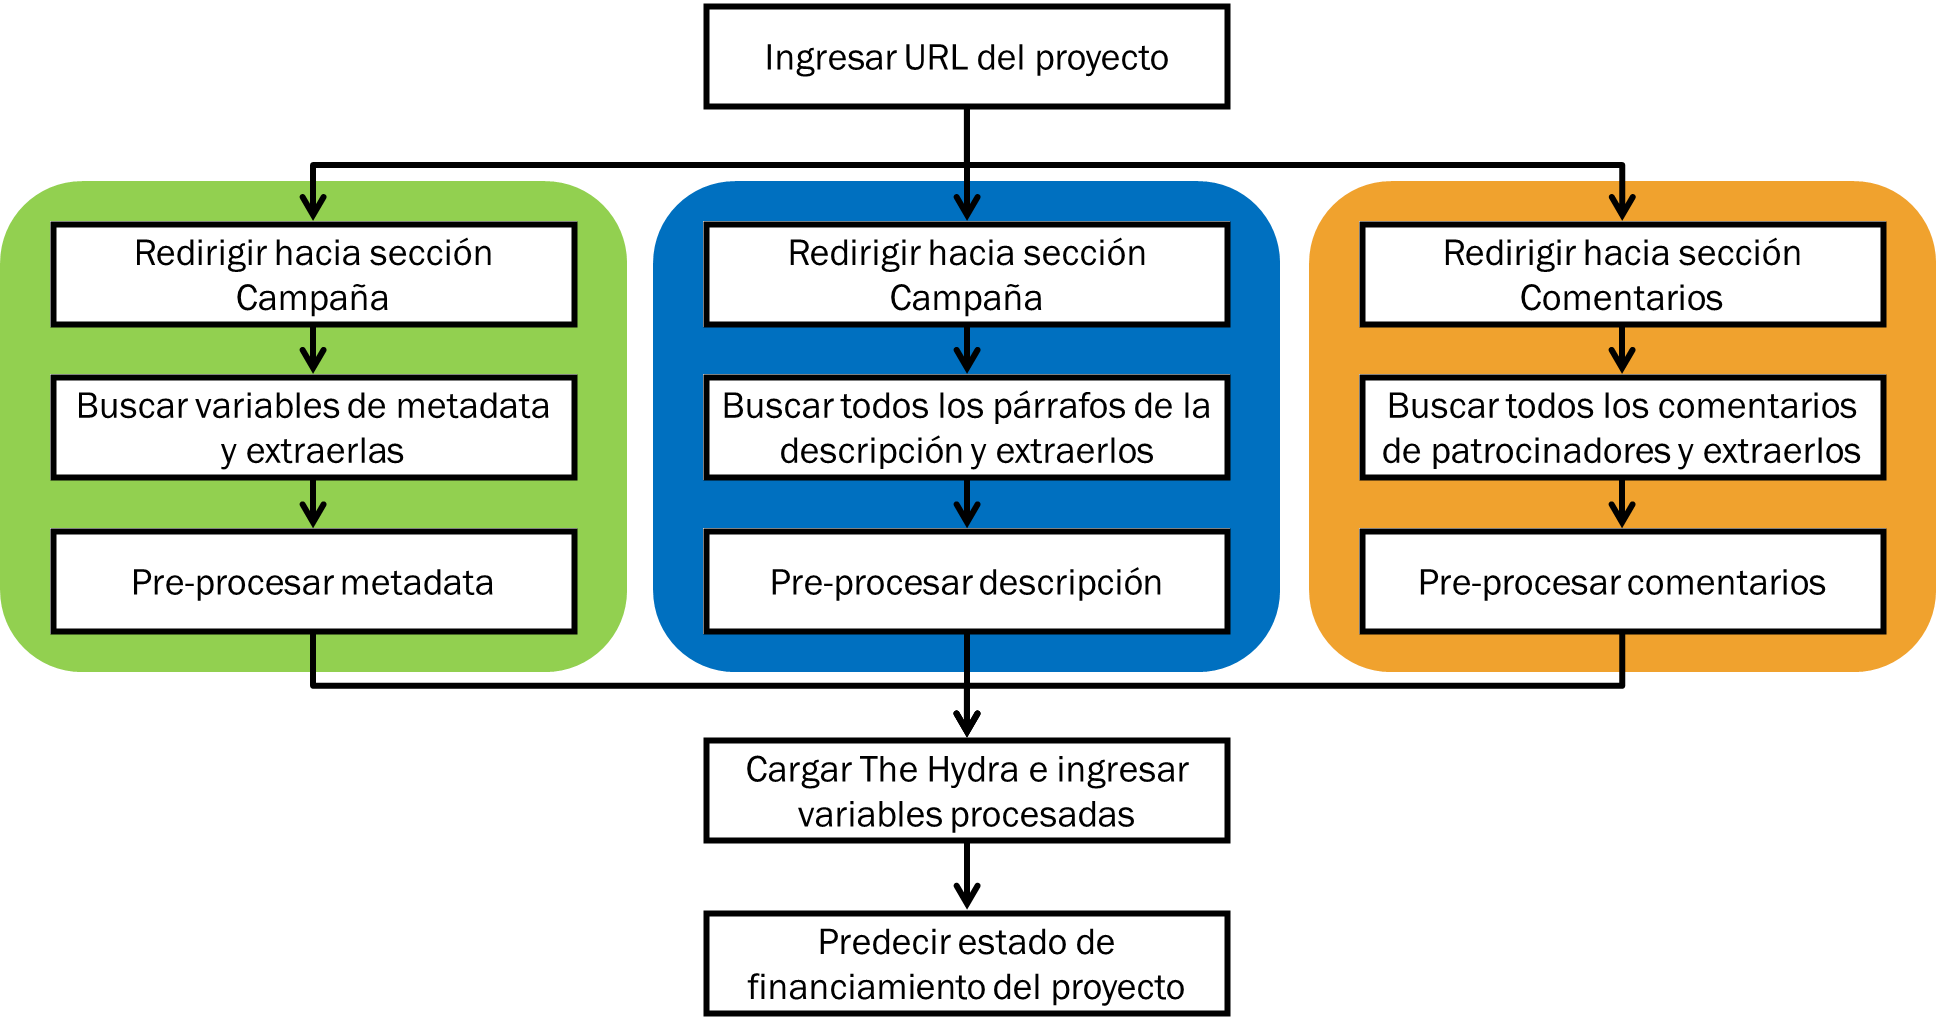
\includegraphics[width=0.95\textwidth]{5/figures/demo_flux.png}
		\caption[Flujograma del sistema piloto]{Flujograma del sistema piloto.\\
		Fuente: Elaboración propia.}
		\label{5:fig13}
	\end{center}
\end{figure}

Como se observa en la anterior imagen, el software ejecutado localmente desde Jupyter Notebook recibe de entrada el enlace web de un proyecto no finalizado de Kickstarter. Uno de los experimentos hechos el 23 de enero del 2021 se realizó con la campaña de la Figura \ref{5:fig14}.

\begin{figure}[!ht]
	\begin{center}
		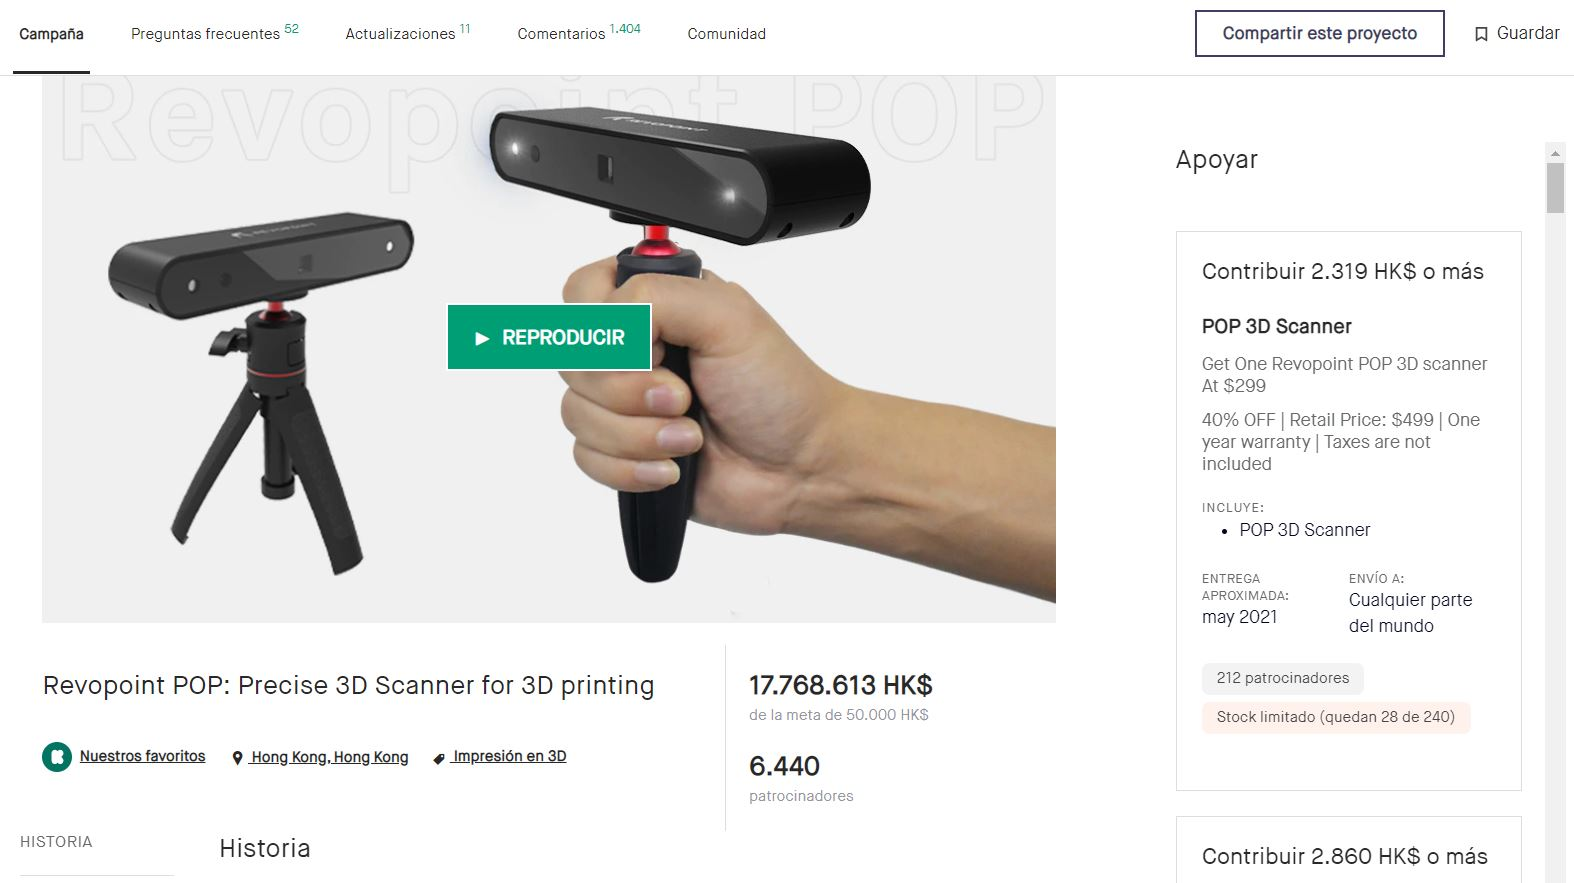
\includegraphics[width=0.75\textwidth]{5/figures/example_project_150221.jpg}
		\caption[Proyecto usado para la demostración. Captura de pantalla: 15/02/21]{Proyecto usado para la demostración. Captura de pantalla: 15/02/21.\\
		Fuente: \cite{ot_kickstarter_revopointproject}}
		\label{5:fig14}
	\end{center}
\end{figure}

La primera acción hecha por el sistema fue extraer la metainformación, descripción y comentarios del proyecto desde el ingreso al URL por un navegador. Debido al cambio de políticas de acceso a la plataforma en 2020, Kickstarter detecta la presencia de bots y restringe la navegación usando CAPTCHAs para evitar su accionar. Algunas veces fue detectado el bot del sistema. Ante ello, la única acción manual por parte del usuario en el sistema se da en este paso presionando por 5 segundos el botón de “\textit{I'm a human}” (Soy humano por su traducción al español) que se muestra en la ventana. Desde este punto, luego de ingresar al enlace de la campaña del proyecto, el sistema primero se redirige a la sección de la metainformación y extrae las variables usadas para el entrenamiento del modelo. Del mismo modo, repite esta secuencia para la descripción y los comentarios.

Los datos extraídos de cada modalidad se muestran en la Figura \ref{5:fig15} respectivamente.
\begin{figure}[!ht]
	\centering
	\small
	\begin{subfigure}{.35\textwidth}
		\centering
		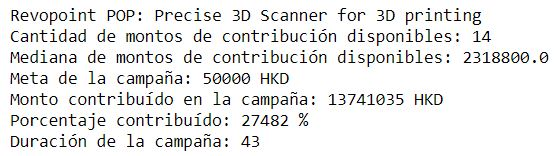
\includegraphics[width=0.95\linewidth]{5/figures/metadata_scraped_project.jpg}
		\caption{Metainformación}
	\end{subfigure}%
	\begin{subfigure}{.35\textwidth}
		\centering
		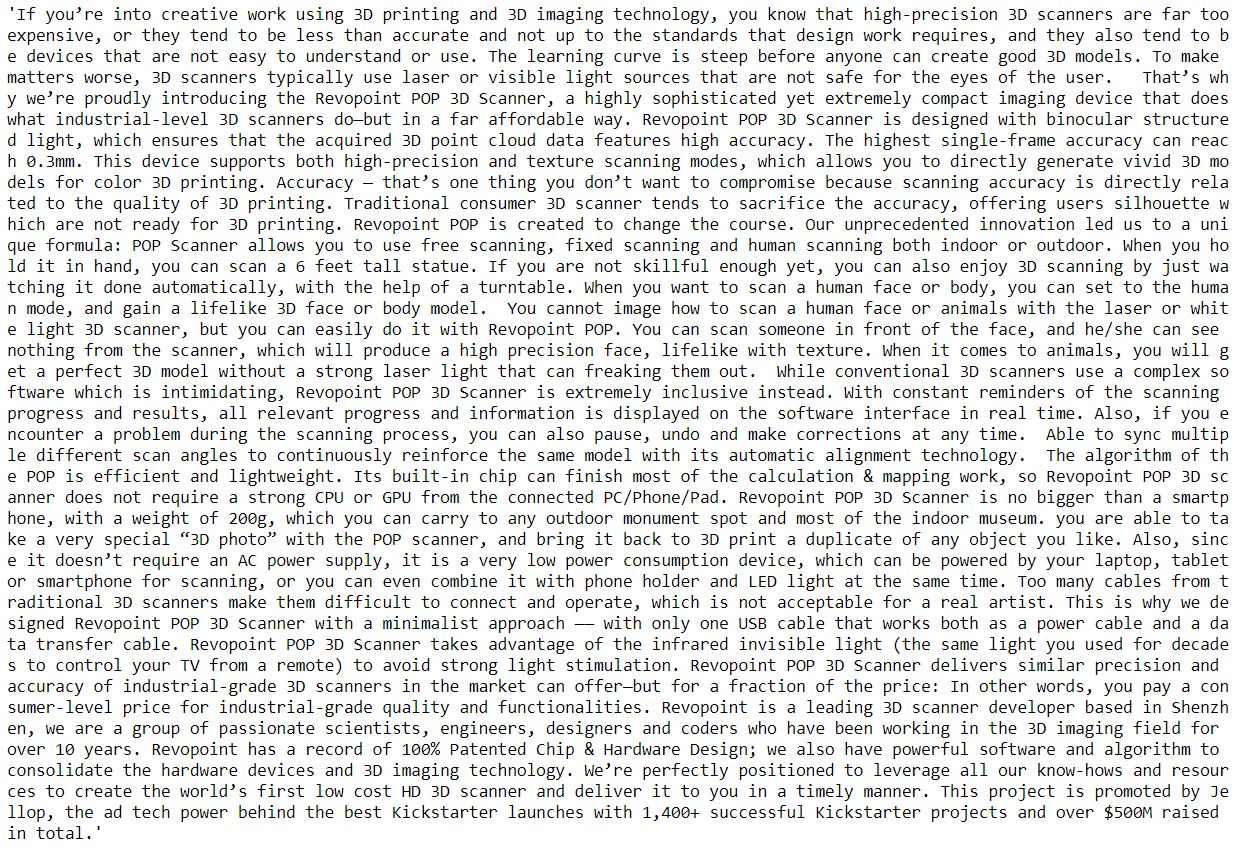
\includegraphics[width=0.95\linewidth]{5/figures/description_scraped_project.jpg}
		\caption{Descripción}
	\end{subfigure}%
	\begin{subfigure}{.35\textwidth}
		\centering
		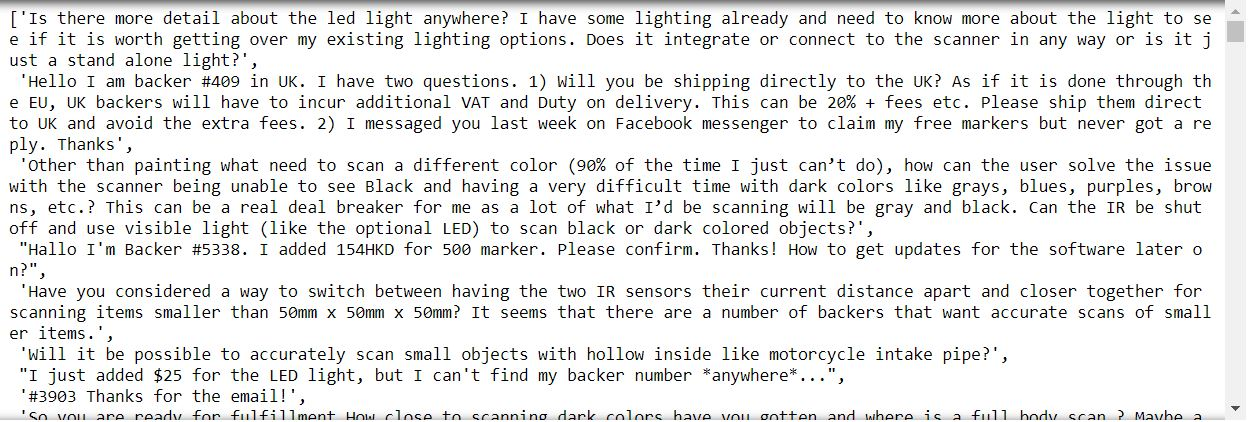
\includegraphics[width=0.95\linewidth]{5/figures/comments_scraped_project.jpg}
		\caption{Comentarios}
	\end{subfigure}
	\caption[Variables extraídas del proyecto ejemplo]{Variables extraídas del proyecto ejemplo.\\
	Fuente: Elaboración propia.}
	\label{5:fig15}
\end{figure}

Esta información es pre-procesada de la misma manera que la data usada para entrenar cada modelo. A continuación, el modelo cargado The Hydra recibe los datos procesados y concatenados para realizar la predicción. Si el umbral es por lo menos 0.50, el resultado será \textbf{EXITOSO} (\textit{Successful} en inglés) como en la Figura \ref{5:fig16}.

\begin{figure}[!ht]
	\begin{center}
		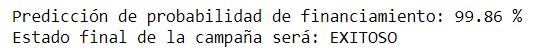
\includegraphics[width=0.70\textwidth]{5/figures/demo_project_prediction.jpg}
		\caption[Resultado de predicción de The Hydra para el proyecto consultado]{Resultado de predicción de The Hydra para el proyecto consultado.\\
		Fuente: Elaboración propia.}
		\label{5:fig16}
	\end{center}
\end{figure}